\chapter{Week 7}

\section{Week 7 Lecture 1}\label{sec:w7lec1}

Consider a large population of units. We are interested in some numerical property of this population, i.e. a \textbf{parameter}. 
This can be an average measurement \(\mu\) (eg. average weight, income, blood pressure, etc.), or a population proportion \(p\) of a certain characteristic (eg. \% of left-handed students at UQ, Australians with a certain disease, etc.).

\bigskip

Suppose a random sample of \(n\) units is taken from our population and a sample \textbf{statistic} is computed. 
This could be a sample area \(\bar{X}\) for quantitative variables, or a sample proportion \(\hat{p}\) for a catergorical variable, etc. \dots

\bigskip

So, the question is, how \textbf{confident} can we be that our sample statistic (i.e. \textbf{point estimate}) is \textbf{close} to our population parameter?

\begin{example}\label{eg:skittlesandmnms}
    Alan presents a jar of skittles and m\&m's prepared by his wife. 
    A student extracts a sample of \(n=75\) from the jar and, to estimate the proportion of skittles, finds a point estimate of \(\hat{p} = \frac{25}{75} = 0.333 = 33.3\%\).
\end{example}

How \textbf{confident} can we be that \(\hat{p}\) is \textbf{close} to the population proportion?

\subsection{Margin of error and level of confidence} \label{subsec:MOE and lvl of conf}

"Closeness" can be formalised as a \textbf{margin of error} (i.e. the error or lack of closeness that you are willing to tolerate). 
"Confidence" can be formalised as a \textbf{"level of condfidence"}. 

\bigskip

Recall from first year statistics that an approximate \(90\%,95\%\) or \(99\%\) \textbf{confidence interval} for \(p\) can be constructed via 

\begin{align*}
    90\% \text{CI} &= \hat{p} \pm 1.64 \times \sqrt{\frac{\hat{p}(1-\hat{p})}{n}},\\
    95\% \text{CI} &= \hat{p} \pm 1.96 \times \sqrt{\frac{\hat{p}(1-\hat{p})}{n}},\\
    99\% \text{CI} &= \hat{p} \pm 2.58 \times \sqrt{\frac{\hat{p}(1-\hat{p})}{n}},\\
\end{align*}

or in general terms 

\begin{align*}
    \text{condfidence level}~ \text{CI} &= \text{point estimate} \pm \text{critical value} \times \text{standard error (se)}\\
    &= \text{point estimate} \pm \text{margin of error (MOE)}.\\
\end{align*}

For our particular sample (see example \ref{eg:skittlesandmnms}), we had \(n=75, \hat{p} = 0.333\), and so we can enumerate our CI:

\begin{align*}
    90\% \text{CI} &= 0.333 \pm 1.64 \times \sqrt{\frac{0.333 \times 0.667}{75}}\\
    &= 0.333 \pm 1.64 \times 0.054\\
    &= 0.333 \pm 0.089\\
    &= (0.244, 0.422) = 24.4\% \text{ and } 42.2\%.
\end{align*}

This means that we can be \(90\%\) confident that the true population proportion lies within the interval \((0.244, 0.422)\). 
We have two questions from this:

\begin{enumerate}
    \item We know that the critical values come from a standard normal distribution, but what does a Normal distribution have to do with a proportion?
    \item Why do these critical values \textit{not} depend on the underlying proportion \(p\)?
\end{enumerate}

\subsection{Pivot quantities}\label{subsec:pivot quants}

\begin{definition}\label{defn:pivot var}
    A \textbf{pivot variable} is a theoretical (\& generally not computable) transformation of a random variable (i.e. data) such that its distribution no longer depends on any unknown parameters. 
\end{definition}

\begin{example}[Pivot variable for Normal data]\label{eg:pivot var normal}
    Let \(X_1,...,X_n \underset{\text{i.i.d.}}{\sim} N(\mu,\sigma^2)\) where \(\mu\) is unknown but \(\sigma^2\) is known (for simplicity). 
    What do we know about the distribution of \(\bar{X} = \frac{X_1,...,X_n}{n}\)?
    \begin{equation*}
        \bar{X}\sim N(\mu,\frac{\sigma^2}{n}).
    \end{equation*}
    Thus, we have a theoretical (\& non-computable) transformation 
    \begin{equation*}
        \frac{\bar{X} - \mu}{\sigma/\sqrt{n}} \sim N(0,1)
    \end{equation*}
    which does \textit{not} depend on any unknown parameters anymore. 
    Hence, \(\frac{\bar{X} - \mu}{\sigma/\sqrt{n}}\) is an example of a pivot variable. 
\end{example}

Pivot variables can be used to construct confidence intervals and hypothesis tests for population parameters. 

\begin{example}[Previous example continued]\label{eg:pivot var normal continued}
    Notice that 
    \begin{align*}
        95\% &= \mathbb{P}(-1.96 \leq N(0,1) \leq 1.96)\\
        &= \mathbb{P}(-1.96 \leq \frac{\bar{X} - \mu}{\sigma/\sqrt{n}} \leq 1.96)\\
        &= \mathbb{P}(-1.96\sigma/\sqrt{n} \leq \bar{X} - \mu \leq 1.96\sigma/\sqrt{n})\\
        &= \mathbb{P}(\bar{X}+1.96\sigma/\sqrt{n} \geq \mu \geq \bar{X}-1.96\sigma/\sqrt{n})\\
    \end{align*}
    This is how the classical 95\% confidence interval for \(\mu\) is derived from first year statistics
    \begin{equation*}
        \bar{X}\pm 1.96\sigma/\sqrt{n}
    \end{equation*}
    is formally derived. 
\end{example}

[tbc]




\section{Week 7 Lecture 2}\label{sec:w7lec2}

Recall:

\begin{itemize}
    \item A \textbf{pivot variable} (or \textbf{pivot quantity}, or simply \textbf{pivot}) is just a theoretical (and non-computable) transformation of a random variable whose distibution no longer depends on any unknown parameters.
    \item Our \textbf{level of confidence} in any estimation procedure must always be tied to some \textbf{margin of error}. 
\end{itemize}

Motivating question: how confident can we be that our sample proportion of \(\hat{p} = 0.333\) of skittles (or disease in our other example) from \hyperref[sec:w7lec1]{Week 7 Lecture 1} is \textit{exactly} the population proportion?
Answer: \(0\%\), since we have not allowed for any MOE. 

\bigskip

But, we can be \(90\%\) confident that our estimate is within

\begin{equation*}
    \pm1.64 \text{se}(\hat{p}) = \pm 1.64 \times 0.054 = \pm 8.9\%
\end{equation*}

of the true population proportion (se is standard error). 
Or, we can be \(99\%\) condfident that it lies within 

\begin{equation*}
    \pm2.58 \text{se}(\hat{p}) = \pm 2.58  \times 0.054 = \pm 13.9\%.
\end{equation*}

For this lecture, we want to investigate a more realistic scenario where both \(\mu\) and \(\sigma^2\) are unknown, since it is a bit unrealistic to have a scenario where we truly know one parameter but not the other. 

\subsection{CI's for \texorpdfstring{\(\mu\)}{mu} when \texorpdfstring{\(\sigma^2\)}{sigma\^2} is unknown} \label{subsec:CI for mu, sigma unknown}

Let \(X_1,...,X_n \overset{\text{i.i.d.}}{\sim} N(\mu,,\sigma^2)\) where both \(\mu\) and \(\sigma^2\) are unknown. 
We have already seen that the MLE of \(\mu\) is 

\begin{equation*}
    \bar{X} = \frac{X_1,...,X_n}{n},
\end{equation*}

which has the distribution 

\begin{equation*}
    \bar{X} \sim N(\mu,\sigma^2/n)
\end{equation*}

and that 

\begin{equation*}
    \frac{\bar{X} - \mu}{\sigma/\sqrt{n}} \sim N(0,1)
\end{equation*}

i.e. the standard normal distribution. 
This gives us the first bit of information which we need. 

\bigskip

We have also seen that the (bias-corrected) MLE for \(\sigma^2\) is 

\begin{equation*}
    s^2 = \frac{1}{n-1}\sum_{i=1}^{n}(X_i - \bar{X})^2,
\end{equation*}

which has the distribution 

\begin{equation*}
    \frac{(n-1)s^2}{\sigma^2} \sim \chi_{(n-1)}^2 = \frac{s^2}{\sigma^2} \sim \frac{\chi_{(n-1)}^2}{(n-1)},
\end{equation*}

giving us our second bit of information. 

\bigskip

Moreover, \(\bar{X}\) and \(s^2\) are independent (wow!), giving us our third bit of information. 
Combining the three bits of information above, let's consider the transformation given by 

\begin{align*}
    T = \frac{\bar{X} - \mu}{s/\sqrt{n}} = \frac{\frac{\bar{X} - \mu}{\sigma/\sqrt{n}}}{s/\sigma} \sim \frac{N(0,1)}{\sqrt{chi}_{(n-1)}^2/(n-1)} = T_{n-1}
\end{align*}

by the definition of the \(t\)-distribution (see Student 1905 paper for proof by brute force).

\bigskip

Thus, \(T\) is a theoretical transformation of our data that has a distribution that no longer depends on any unknown parameters \(\mu\) or \(\sigma^2\). 
Hence, from the three bits of info, \(T\) is a \textbf{pivot variable}. 

Like the standard normal distribution, \(t\) distributions are also symmetric and somewhat bell-curved. 

\begin{figure}[H]
    \centering
    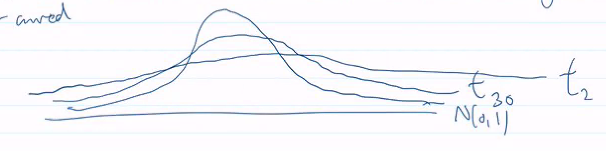
\includegraphics[width=\textwidth]{w7lec2fig1.png}
    \caption{Shape of SND compared to \(t\) distribution}
    \label{fig:shape of SND, t dist}
\end{figure}

To construct \((1-\alpha)100\%\) CI for \(\mu\) when \(\sigma^2\) is also unknown, we again appeal to a known probability statement:

\begin{align*}
    (1-\alpha)100\% &= \mathbb{P}(-t^{\left(1-\frac{\alpha}{2}\right)} \leq T_{n-1} \leq t^{\left(1-\frac{\alpha}{2}\right)})\\
    &= \mathbb{P}(-t^{\left(1-\frac{\alpha}{2}\right)} \leq \frac{\bar{X} - \mu}{s/\sqrt{n}} \leq t^{\left(1-\frac{\alpha}{2}\right)})\\
    &\vdots\\
    &= \mathbb{P}(\bar{X} + t^{\left(1-\frac{\alpha}{2}\right)}s/\sqrt{n} \geq \mu \geq \bar{X} - t^{\left(1-\frac{\alpha}{2}\right)}s/\sqrt{n})\\
\end{align*}

This is the familiar \(\bar{X} + t^{\left(1-\frac{\alpha}{2}\right)}s/\sqrt{n}\) confidence intervals are formally constructed. 

\bigskip

How do we find the cutoffs \(t^{\left(1-\frac{\alpha}{2}\right)}\)? 
We can appeal to tabales, but tables are limited as they will not have every combination of degrees-of-freedom and confidence level that we want. 
So, it's much better to use software. 
For example, suppose we have a sample size of \(n=42\) (df = 41), which does not normally appear in a table, and a confidence level of \(97\%\); 
what is the required \(t_{41}^{0.985}\)? In R,

\medskip 

\begin{lstlisting}
    > qt(0.985, 41)
    [1]     2.248
\end{lstlisting}

\medskip

So, a \(97\%\) CI for \(\mu\) when \(\sigma^2\) is unknown for \(n=42\) samples can be constructed via 

\begin{equation*}
    \bar{X} \pm 2.248s/\sqrt{n}
\end{equation*}

C.f. first year stats.

---

Not all distributions are symmetric, so not all confidence intervals are symmetric around the point estimate. 
Indeed, not all CIs are additive (\(\pm\)) in their margins of errors. Some CIs have multiplicative (i.e. relative) MOEs.

\subsection{CI's for a population variance \texorpdfstring{\(\sigma^2\)}{sigma\^2}} \label{subsec:CI for sigma}

Let \(X_1,...,X_n \overset{\text{i.i.d.}}{\sim} N(\mu,,\sigma^2)\) where both \(\mu\) and \(\sigma^2\) are unknown. 
We have already seen that 

% \begin{align*}
    
% \end{align*} 

and so \(\frac{(n-1)s^2}{\sigma^2}\) is a \textbf{pivot}. 

The \(\chi^2\) distributions are \textbf{not symmetric} and look like this:

[fig2]